\apendice{Especificación de Requisitos}

\section{Introducción}
En el apéndice actual se detallarán los requisitos funcionales y no funcionales considerados durante el desarrollo de InteraDD, 
derivados de los objetivos planteados en el capítulo 2 de la memoria del proyecto. Además se describirán también los principales casos de uso y los 
prototipos de la interfaz implementada.

\section{Requisitos}
\subsection*{Requisitos funcionales}
En la Tabla \ref{tab:funcionales} se recogen los principales requisitos funcionales definidos para InteraDD. Estos requisitos describen las funcionalidades que la aplicación debe proporcionar al usuario para cumplir los objetivos planteados en el proyecto.
\begin{table}[ht]
\centering
\begin{tabularx}{\textwidth}{c X}
\toprule
\textbf{Código} & \textbf{Descripción} \\
\midrule
RF-01 & Permitir al usuario seleccionar dos principios activos para realizar el análisis de interacción farmacológica. \\

RF-02 & Detectar el nivel de interacción farmacológica entre los principios activos seleccionados mediante el análisis de las enzimas del sistema CYP450. \\

RF-03 & Mostrar el nivel de riesgo de la interacción clasificándolo como \textit{Low}, \textit{Medium} o \textit{High}. \\

RF-04 & Mostrar una explicación del mecanismo farmacocinético responsable de la interacción detectada. \\

RF-05 & Permitir consultar las enzimas metabólicas principales asociadas a cada principio activo. \\

RF-06 & Mostrar el papel desempeñado por cada principio activo sobre las enzimas compartidas (sustrato, inhibidor o inductor), cuando dicha información esté disponible. \\

RF-07 & Representar gráficamente los efectos adversos asociados a los principios activos consultados. \\

RF-08 & Proponer alternativas terapéuticas compatibles cuando la interacción detectada sea de riesgo medio o alto. \\

RF-09 & Informar al usuario cuando no exista información suficiente para realizar alguna de las consultas solicitadas. \\

RF-10 & Mantener visibles los resultados obtenidos hasta que el usuario realice una nueva búsqueda. \\
\bottomrule
\end{tabularx}
\caption{Requisitos funcionales de InteraDD.}
\label{tab:funcionales}
\end{table}

\subsection*{Requisitos no funcionales}
La Tabla \ref{tab:no funcionales} muestra los requisitos no funcionales considerados durante el desarrollo de InteraDD. Estos requisitos establecen las características de calidad que debe cumplir el sistema, como la usabilidad, el rendimiento, la mantenibilidad, la compatibilidad y la fiabilidad, garantizando un funcionamiento adecuado de la herramienta desarrollada.
\begin{table}[ht]
\centering
\begin{tabularx}{\textwidth}{c X}
\toprule
\textbf{Código} & \textbf{Descripción} \\
\midrule
RNF-01 & La aplicación deberá presentar una interfaz web intuitiva y de fácil utilización para el personal sanitario. \\

RNF-02 & El sistema deberá ejecutarse desde un navegador web sin requerir la instalación de software adicional por parte del usuario. \\

RNF-03 & La aplicación deberá proporcionar una respuesta en un tiempo razonable para consultas habituales. \\

RNF-04 & La arquitectura del sistema deberá permitir la incorporación de nuevos principios activos, enzimas y bases de datos sin modificar significativamente la lógica del algoritmo. \\

RNF-05 & El código fuente deberá estar organizado de forma modular para facilitar su mantenimiento y evolución. \\

RNF-06 & La información mostrada deberá proceder de fuentes biomédicas reconocidas y actualizadas (DrugBank, CIMA y SIDER). \\

RNF-07 & El sistema deberá garantizar la trazabilidad de los datos utilizados para justificar el nivel de interacción mostrado. \\

RNF-08 & La aplicación deberá ser compatible con los principales navegadores web modernos. \\

RNF-09 & El sistema deberá mostrar mensajes informativos cuando una consulta no pueda resolverse por ausencia de información. \\

RNF-10 & La aplicación deberá permitir su despliegue en plataformas de computación en la nube para facilitar su acceso y evaluación. \\
\bottomrule
\end{tabularx}
\caption{Requisitos no funcionales de InteraDD.}
\label{tab:no funcionales}
\end{table}

\section{Diagrama de casos de uso}
La Figura \ref{fig:casos} muestra el diagrama de casos de uso para InteraDD. El actor sería el profesional sanitario 
que interactúa con la herramienta introduciendo los principios activos, buscando la interacción entre ambos 
y consultando de esta manera su nivel de interacción, las explicaciones pertinentes, los efectos adversos y las 
alternativas terapéuticas.
\begin{figure}[ht]
    \centering
    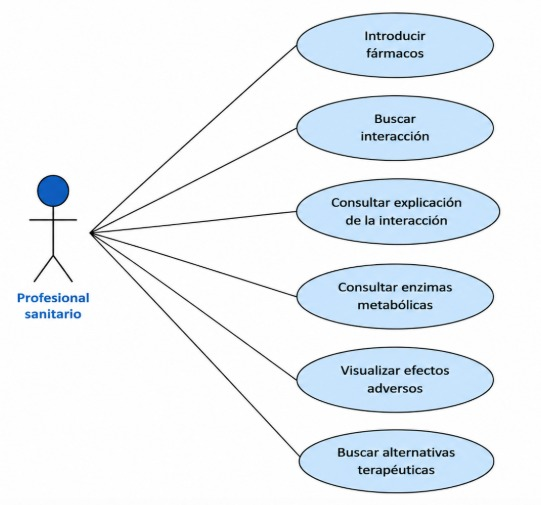
\includegraphics[width=0.45\textwidth]{img/casos uso.png} 
    \caption{Diagrama de casos de uso para InteraDD. Elaboración propia.}
    \label{fig:casos}
\end{figure}


\section{Explicación casos de uso.}
En este apartado se presentan los cinco casos de uso principales de la herramienta desarrollada.
Se encuentran recogidos en las siguientes tablas \ref{tab:CU1} \ref{tab:CU2} \ref{tab:CU3} \ref{tab:CU4} \ref{tab:CU5} 
\begin{table}[ht]
	\centering
	\begin{tabularx}{\linewidth}{ p{0.25\columnwidth} p{0.68\columnwidth} }
		\toprule
		\textbf{CU-1} & \textbf{Buscar interacción farmacológica}\\
		\toprule
		\textbf{Autor} & Profesional sanitario\\
		\textbf{RF asociados} & RF-01, RF-02, RF-03 y RF-10\\
		\textbf{Descripción} & Permite al usuario analizar la posible interacción farmacológica entre dos principios activos seleccionados.\\
		\textbf{Precondición} & El usuario ha seleccionado dos principios activos disponibles en la aplicación.\\
		\textbf{Acciones} &
		\begin{enumerate}
			\item Seleccionar el primer principio activo.
			\item Seleccionar el segundo principio activo.
			\item Pulsar el botón \textit{Search Interaction}.
			\item El sistema analiza las enzimas metabólicas implicadas.
			\item Se calcula el nivel de riesgo.
			\item Se muestran los resultados.
		\end{enumerate}\\
		\textbf{Postcondición} & Se presenta el nivel de interacción junto con la información asociada.\\
		\textbf{Excepciones} & Alguno de los medicamentos no dispone de información suficiente en la base de datos.\\
		\bottomrule
	\end{tabularx}
	\caption{CU-1 Buscar interacción farmacológica.}
	\label{tab:CU1}
\end{table}
\begin{table}[ht]
	\centering
	\begin{tabularx}{\linewidth}{ p{0.25\columnwidth} p{0.68\columnwidth} }
		\toprule
		\textbf{CU-2} & \textbf{Consultar explicación de enzimas}\\
		\toprule
		\textbf{Autor} & Profesional sanitario\\
		\textbf{RF asociados} & RF-05, RF-06\\
		\textbf{Descripción} & Permite visualizar las enzimas CYP450 implicadas en el metabolismo de los principios activos seleccionados.\\
		\textbf{Precondición} & Se ha realizado previamente una búsqueda de interacción.\\
		\textbf{Acciones} &
		\begin{enumerate}
			\item Pulsar el botón \textit{Explain Enzymes}.
			\item El sistema recupera la información almacenada.
			\item Se muestran las enzimas metabólicas principales y el papel de cada fármaco.
		\end{enumerate}\\
		\textbf{Postcondición} & El usuario visualiza la explicación correspondiente.\\
		\textbf{Excepciones} & No existe información enzimática disponible para alguno de los principios activos.\\
		\bottomrule
	\end{tabularx}
	\caption{CU-2 Consultar explicación de enzimas.}
	\label{tab:CU2}
\end{table}
\begin{table}[ht]
	\centering
	\begin{tabularx}{\linewidth}{ p{0.25\columnwidth} p{0.68\columnwidth} }
		\toprule
		\textbf{CU-3} & \textbf{Consultar explicación de la interacción}\\
		\toprule
		\textbf{Autor} & Profesional sanitario.\\
		\textbf{RF asociados} & RF-04\\
		\textbf{Descripción} & Permite conocer el mecanismo biológico responsable de la interacción detectada.\\
		\textbf{Precondición} & Se ha realizado previamente una búsqueda de interacción.\\
		\textbf{Acciones} &
		\begin{enumerate}
			\item Pulsar el botón \textit{Explain Interaction}.
			\item El sistema analiza la clasificación obtenida.
			\item Se muestra una explicación textual del mecanismo de interacción.
		\end{enumerate}\\
		\textbf{Postcondición} & El usuario comprende el motivo de la clasificación obtenida.\\
		\textbf{Excepciones} & No existe información suficiente para justificar la interacción.\\
		\bottomrule
	\end{tabularx}
	\caption{CU-3 Consultar explicación de la interacción.}
	\label{tab:CU3}
\end{table}
\begin{table}[ht]
	\centering
	\begin{tabularx}{\linewidth}{ p{0.25\columnwidth} p{0.68\columnwidth} }
		\toprule
		\textbf{CU-4} & \textbf{Consultar efectos adversos}\\
		\toprule
		\textbf{Autor} & Profesional sanitario\\
		\textbf{RF asociados} & RF-07\\
		\textbf{Descripción} & Permite visualizar los efectos adversos asociados a los principios activos seleccionados mediante un gráfico interactivo.\\
		\textbf{Precondición} & Se ha realizado previamente una búsqueda de interacción.\\
		\textbf{Acciones} &
		\begin{enumerate}
			\item Pulsar el botón \textit{Side Effects}.
			\item El sistema consulta la base de datos SIDER.
			\item Se genera el gráfico con los efectos adversos encontrados.
		\end{enumerate}\\
		\textbf{Postcondición} & El usuario visualiza los efectos adversos disponibles.\\
		\textbf{Excepciones} & No existen efectos adversos registrados para alguno de los principios activos.\\
		\bottomrule
	\end{tabularx}
	\caption{CU-4 Consultar efectos adversos.}
	\label{tab:CU4}
\end{table}
\begin{table}[ht]
	\centering
	\begin{tabularx}{\linewidth}{ p{0.25\columnwidth} p{0.68\columnwidth} }
		\toprule
		\textbf{CU-5} & \textbf{Buscar alternativas terapéuticas}\\
		\toprule
		\textbf{Autor} & Profesional sanitario\\
		\textbf{RF asociados} & RF-08\\
		\textbf{Descripción} & Permite consultar principios activos alternativos pertenecientes al mismo grupo ATC y con menor riesgo de interacción.\\
		\textbf{Precondición} & Se ha realizado previamente una búsqueda de interacción.\\
		\textbf{Acciones} &
		\begin{enumerate}
			\item Pulsar el botón \textit{Alternatives}.
			\item El sistema consulta el grupo ATC correspondiente.
			\item Se muestran las alternativas disponibles.
		\end{enumerate}\\
		\textbf{Postcondición} & El usuario obtiene posibles alternativas terapéuticas.\\
		\textbf{Excepciones} & No existen alternativas disponibles para el principio activo seleccionado.\\
		\bottomrule
	\end{tabularx}
	\caption{CU-5 Buscar alternativas terapéuticas.}
	\label{tab:CU5}
\end{table}
